\section{Evaluation and Results}
In our work, we compare different state-of-the-art CSSL methods in different setups (see Appx.~\ref{appx:setup} for details regarding our evaluation setup).

\subsubsection{Performance Comparison against CSSL}

Here, we focus on the overall performance of Kaizen, CaSSLe and the \emph{No distill} setup. In Fig.~\ref{fig:general_performance_comparison}, we present a comparative analysis of Continual Accuracy and Final Accuracy across various methods, each employing different (SSL) models for the feature extractor. This comparison is specifically conducted on the WISDM2019 dataset, which has been divided into six equal-sized tasks. We observe that Kaizen consistently surpasses the two baseline models across all evaluation metrics and SSL methods. Specifically, using BYOL, Kaizen achieved the highest continual accuracy (0.588) and final accuracy (0.481), exceeding CaSSLe by 0.098 and 0.071, respectively. Notably, data availability is standardized across methods, with each having access to current task data and 1\% replay data from previous tasks. Kaizen's superiority is attributed to integrating knowledge distillation and fine-tuning into the pipeline, rather than solely training the classifier at the end.

\subsubsection{Performance Variation across Time}

\begin{figure}
    \centering
    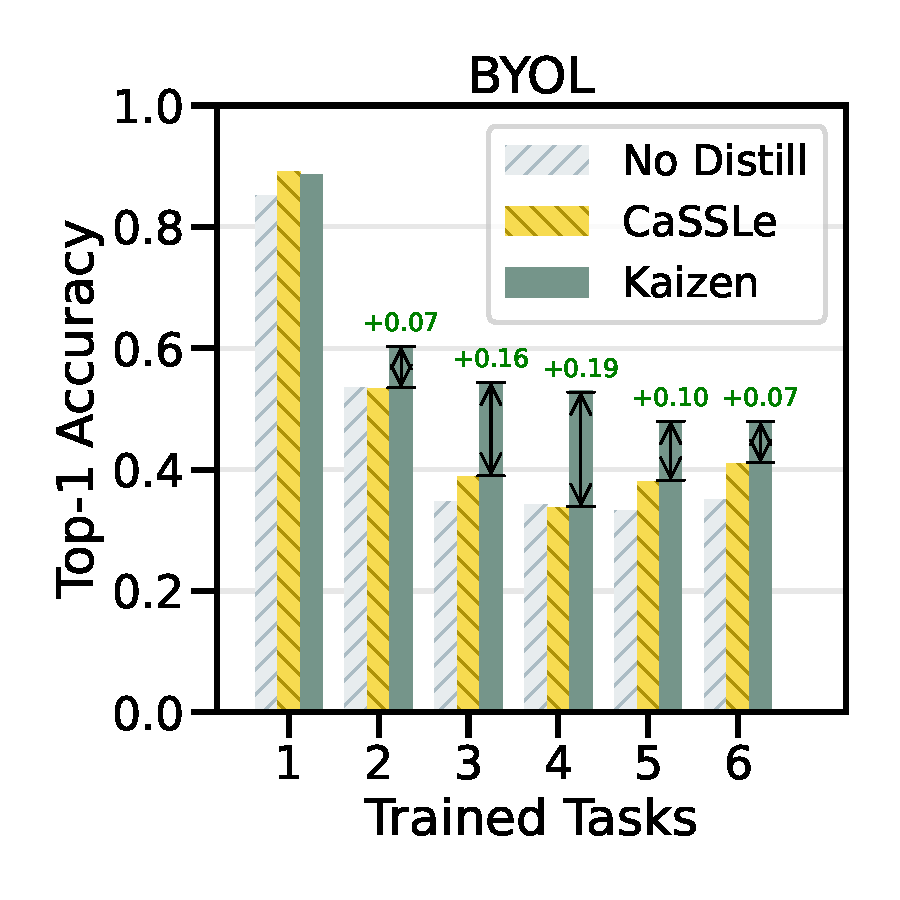
\includegraphics[width=0.49 \linewidth ]{figures_new/Part_1/F3-WISDM2019-BYOL-6Tasks-v2.pdf}
    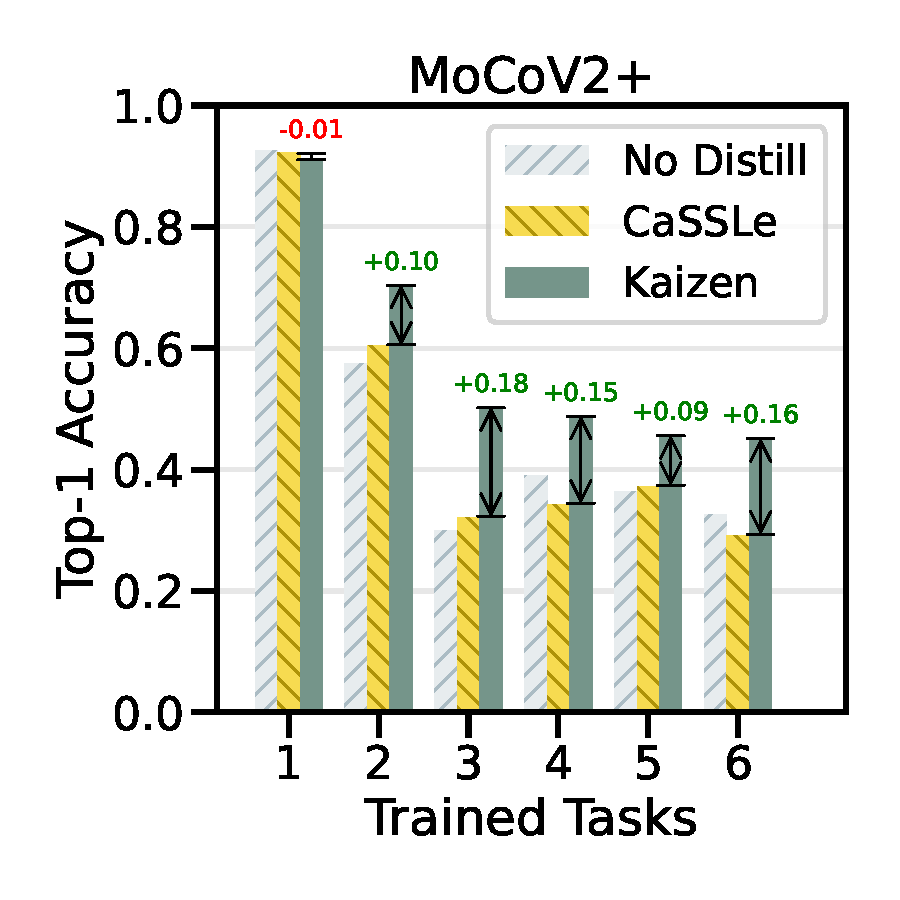
\includegraphics[width=0.49 \linewidth ]{figures_new/Part_1/F3-WISDM2019-MoCoV2+-6Tasks-v2.pdf}
    \vspace{-0.2in}
    \caption{Average performance over tasks on WISDM2019. Comparison is drawn between training methods using different SSL algorithms across different tasks.}
        \vspace{-0.1in}
    \label{fig:performance_across_time_cifar}
\end{figure}

In this evaluation, we examine the performance of different methods at different stages of the continual learning process. Fig.~\ref{fig:performance_across_time_cifar} shows the average accuracy over trained tasks of Kaizen, CaSSLe and \emph{No distill} after training on each task. We find that in general, all methods show lower performance after training on more tasks, partially because the classification problem becomes more difficult as the number of classes increases, as well as catastrophic forgetting. Echoing the results of the previous evaluation, Kaizen maintains a higher level of accuracy overall, even though all methods start from similar performance on the first task.


\subsubsection{Per-task Performance Breakdown} \label{subsection:per_task} 
\begin{figure}[t]
    \centering
    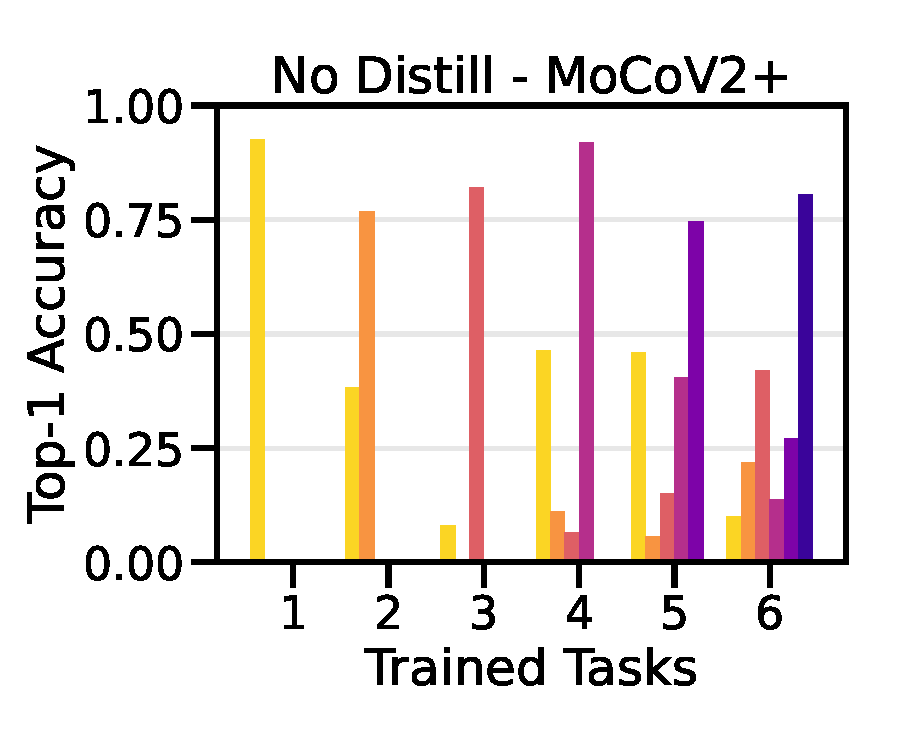
\includegraphics[width=0.32 \linewidth ]{figures_new/Part_1/F4-WISDM2019-NoDistill-MoCoV2+-6Tasks-v2.pdf}
    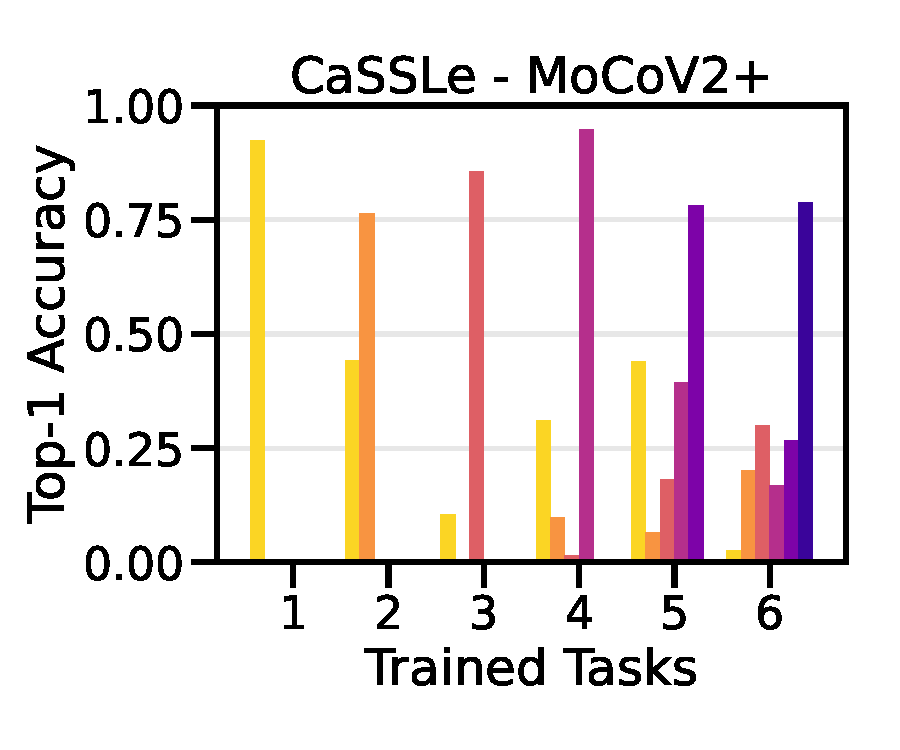
\includegraphics[width=0.32 \linewidth ]{figures_new/Part_1/F4-WISDM2019-CaSSLe-MoCoV2+-6Tasks-v2.pdf}
    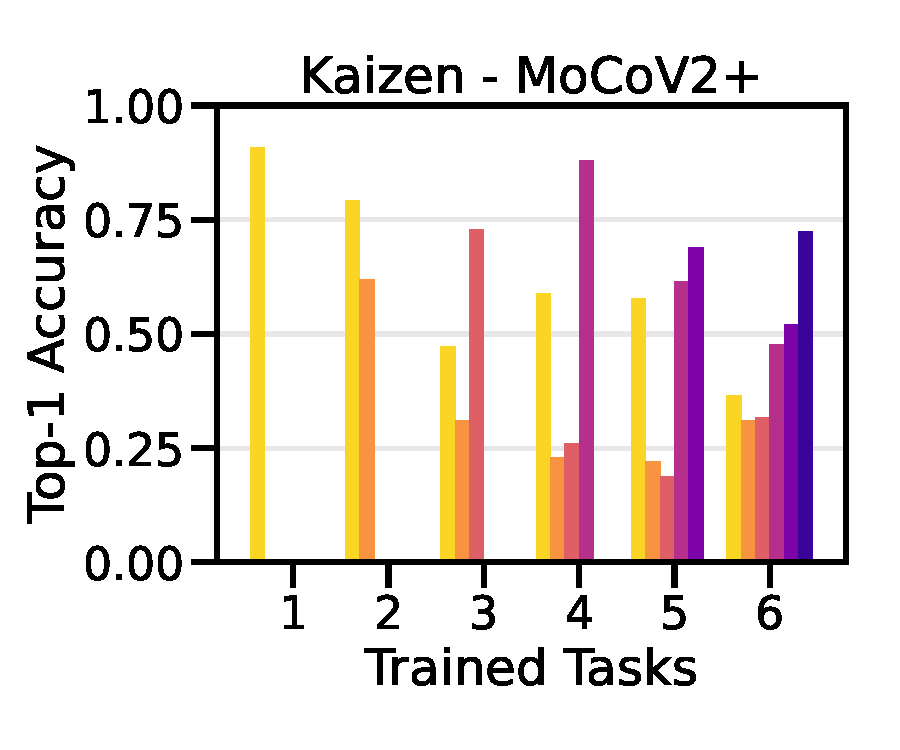
\includegraphics[width=0.32 \linewidth ]{figures_new/Part_1/F4-WISDM2019-Ours-MoCoV2+-6Tasks-v2.pdf} \\
    \vspace{-0.05in}
    
    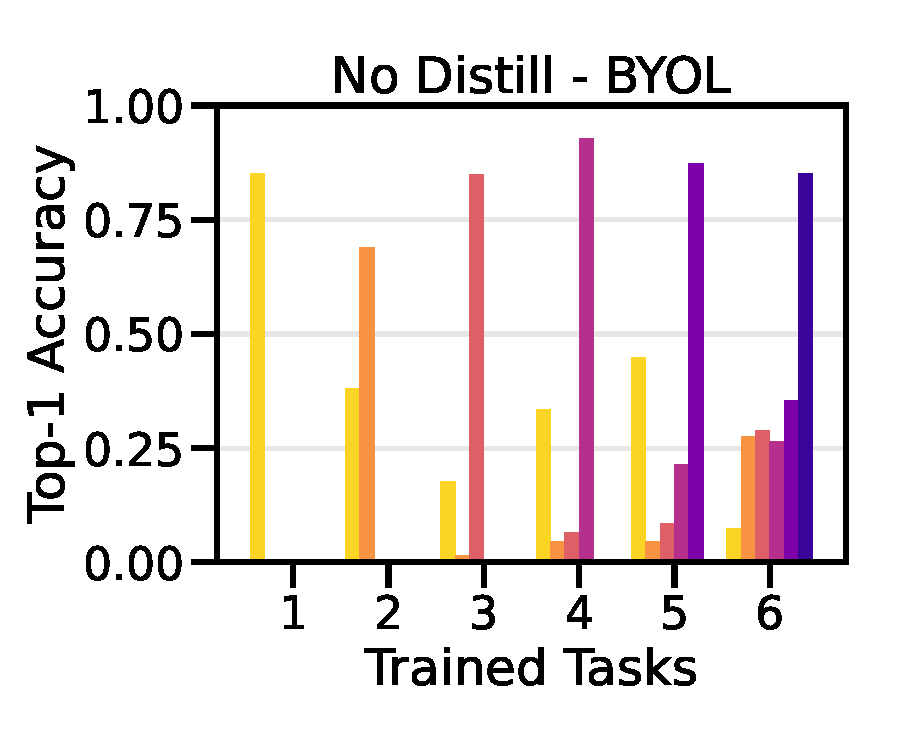
\includegraphics[width=0.32 \linewidth ]{figures_new/Part_1/F4-WISDM2019-NoDistill-BYOL-6Tasks-v2.pdf}
    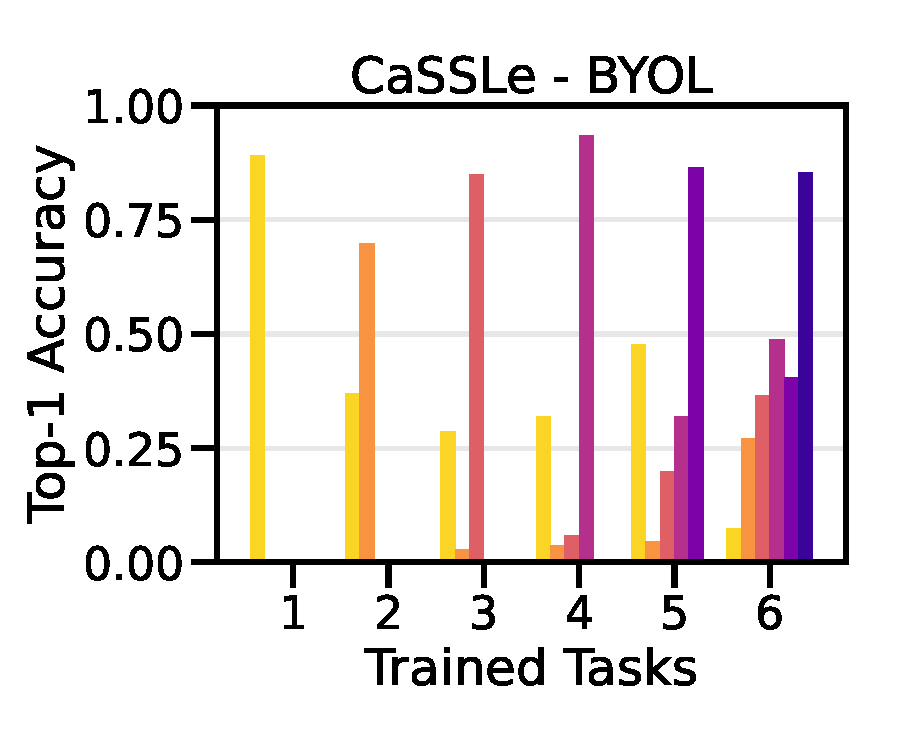
\includegraphics[width=0.32 \linewidth ]{figures_new/Part_1/F4-WISDM2019-CaSSLe-BYOL-6Tasks-v2.pdf}
    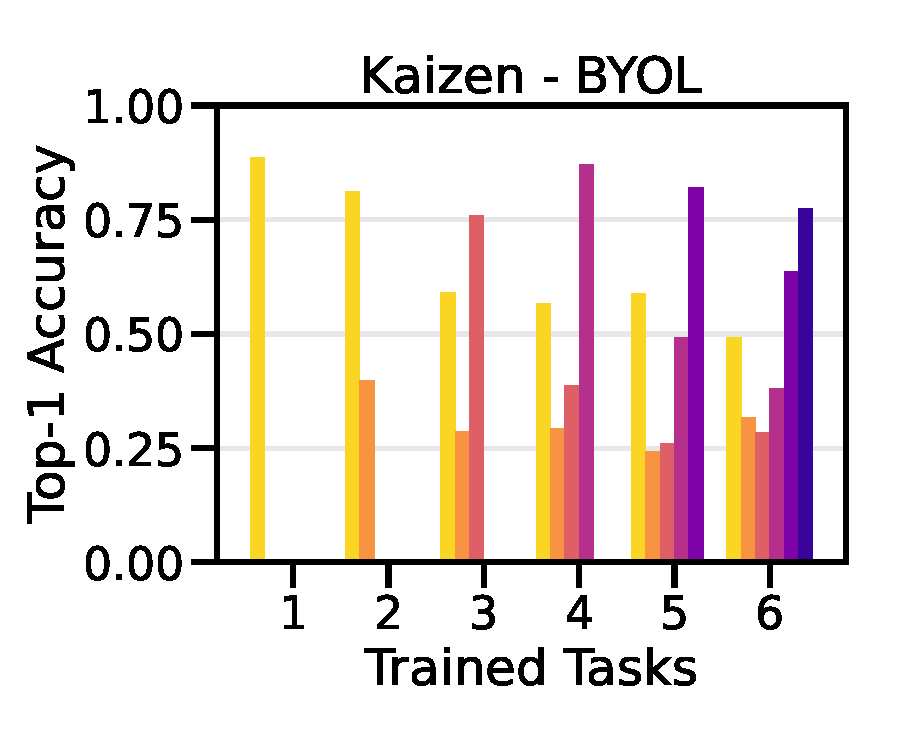
\includegraphics[width=0.32 \linewidth ]{figures_new/Part_1/F4-WISDM2019-Ours-BYOL-6Tasks-v2.pdf} \\
    \vspace{-0.05in}
    
\includegraphics[width=0.65 \linewidth ]{figures_new/Part_1/F4-WISDM2019-6Tasks-v2_legend.pdf}
    \vspace{-0.1in}
    
    \caption{Detailed breakdown of performance over tasks on WISDM2019. Fine-grained accuracy for every task is shown.}
        
    \label{fig:performance_per_task}
\end{figure}

\begin{table}[t!]
\caption{SSL and baseline performance comparison. We evaluate three continual learning strategies across four metrics on WISDM2019. Kaizen with BYOL outperforms in most metrics. The best performance for a SSL method is bolded, and that across SSL methods is underlined. (FA: Final Accuracy, CA: Continual Accuracy, F: Forgetting, FT: Forward Transfer).}

\begin{center}
\small
\begin{tabularx}{\linewidth}{c!{\vrule width 1.5pt}c!{\vrule width 1.5pt}*{4}c}

\textbf{SSL}        &     \textbf{Baseline}     & \textbf{FA} $\uparrow$ & \textbf{CA} $\uparrow$ & \textbf{F} $\downarrow$ & \textbf{FT} $\uparrow$ \\
\hline \hline
\multirow{3}{*}{BYOL}    & No Distill & 0.351          & 0.460              & 0.587          & 0.006            \\
                         & CaSSLe     & 0.410          & 0.490              & 0.527          & \textbf{0.008}   \\
                         & Kaizen       & \textbf{\underline{0.481}} & \textbf{\underline{0.588}}     & \textbf{\underline{0.408}} & -0.107           \\ \hline
\multirow{3}{*}{MoCoV2+}  & No Distill & 0.326          & 0.480              & 0.606          & 0.007            \\
                         & CaSSLe     & 0.292          & 0.476              & 0.662          & \textbf{\underline{0.023}}   \\
                         & Kaizen       & \textbf{0.453} & \textbf{0.586}     & \textbf{0.401} & -0.077           \\
\end{tabularx}
    \vspace{-0.2in}
\end{center}

\label{tab:ssl_baseline}
\end{table}
Kaizen prioritises knowledge retention over the acquisition of new task proficiency. This is evidenced through an analysis of per-task performance at sequential stages, as depicted in Fig. \ref{fig:performance_per_task}. Here, the performance metrics of the models on individual tasks are evaluated through the continual learning process, utilizing MoCoV2+ and BYOL as the self-supervised learning method. Notably, Kaizen demonstrates more graceful knowledge forgetting in comparison to CaSSLe, where there is a gradual decline in performance on prior tasks. While CaSSLe excels in adapting to new tasks, it shows a significant and rapid deterioration in performance on previously learned tasks. Kaizen demonstrated a more balanced trade-off between mastering new tasks and retaining knowledge from past tasks.


\subsubsection{Comprehensive Evaluation of Continual Learning and SSL Methods}

Table \ref{tab:ssl_baseline} presents the performance of Kaizen, CaSSLe and \emph{No Distill} on different metrics. These results show that Kaizen achieved the best performance in terms of the final and continual accuracy. 
As expected, the absence of distillation from the \emph{No Distill} approach hurts the accuracy of the overall continual learning framework as it is unable to maintain knowledge with each additional task. This can also be seen in the Forgetting metric where \emph{No Distill} is 0.179 higher than Kaizen and 0.06 higher than CaSSLe when BYOL is used as the SSL method. BYOL in general performs better as the contrastive learning and knowledge retention mechanism compared to MoCoV2+. On the other hand, as shown in the results above, CaSSLe and \emph{No Distill}, show a slight positive forward transfer in some cases, while Kaizen suffers from a negative forward transfer. This can be explained by the tendencies of CaSSLe and \emph{No Distill} prioritising learning from new data and outperforming specialised models.

\subsubsection{Influence of the Importance Coefficient for Continual Fine-tuning}

As introduced in Section~\ref{subsec:balancing}, the importance coefficient $\lambda_{\mathrm{C}}$ specifies the relative importance of the knowledge distillation task compared to learning from new data. As such, it can have a direct impact on the performance of the classifier across time: a higher importance coefficient forces the model to focus on knowledge retention, while a lower coefficient shifts this focus to new task learning.

\begin{figure}[t]
\begin{center}
   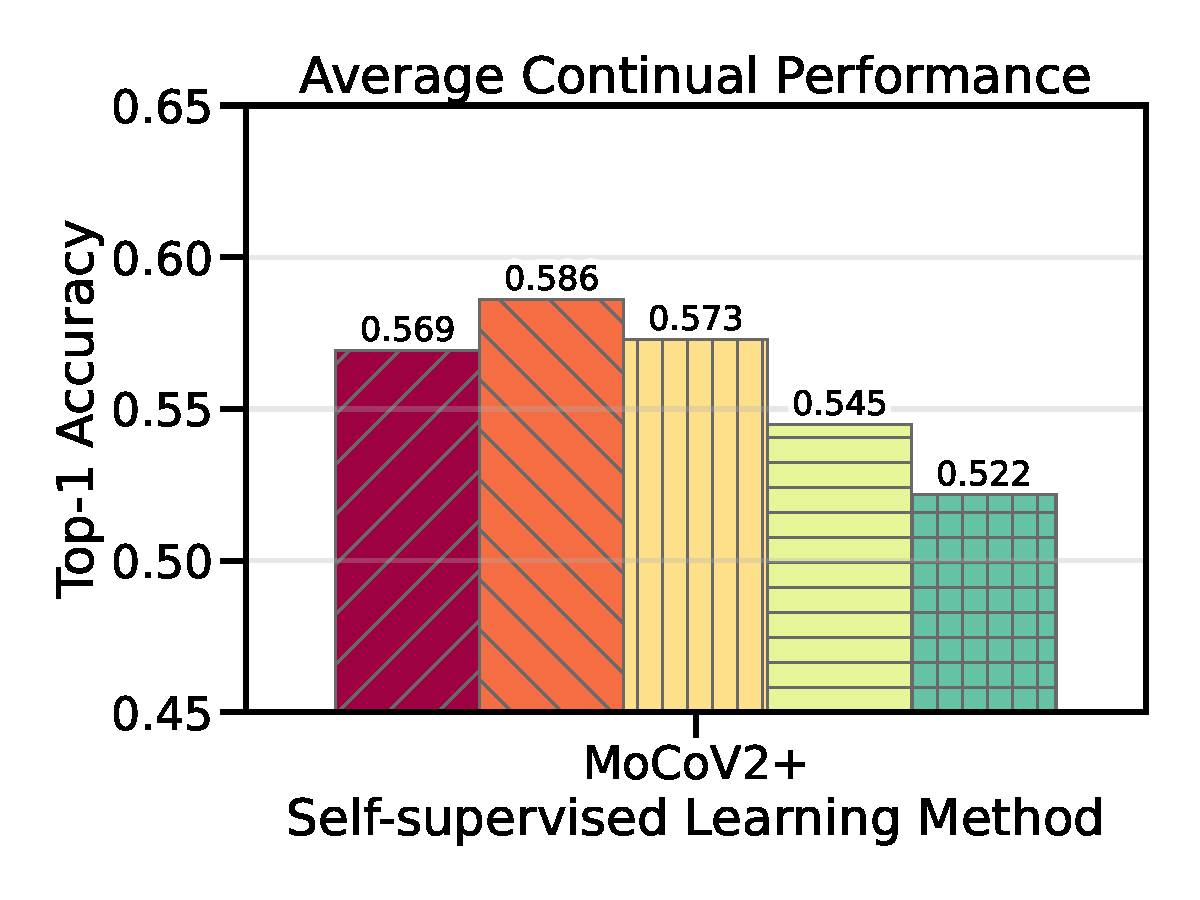
\includegraphics[width=0.49\linewidth]{figures_new/Part_2/F1-WISDM2019-6Tasks-Continual_Accuracy-v2.pdf}
   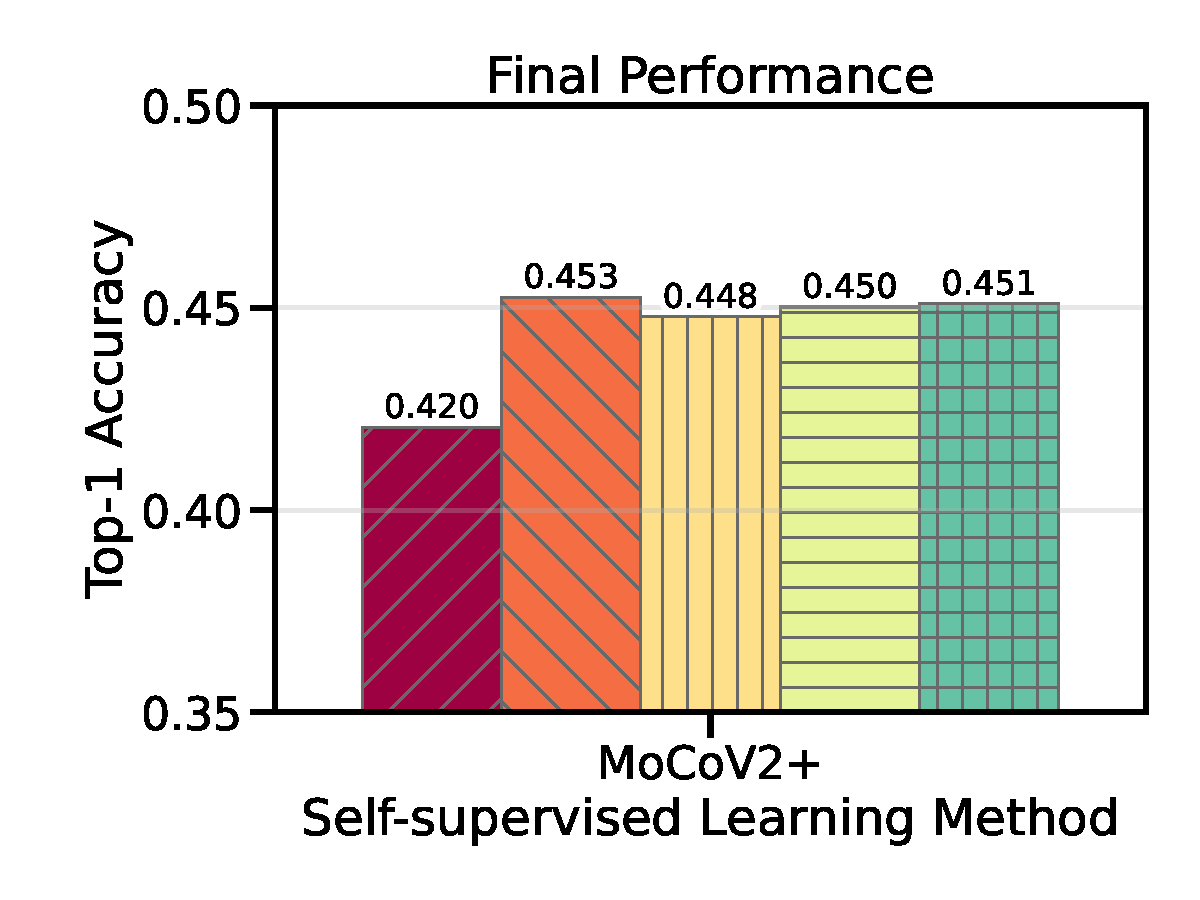
\includegraphics[width=0.49\linewidth]{figures_new/Part_2/F1-WISDM2019-6Tasks-Final_Accuracy-v2.pdf} \\
   \vspace{-0.05in}
   
\includegraphics[width=0.8\linewidth]{figures_new/Part_2/F1-WISDM2019-6Tasks-v2_legend.pdf}
\end{center}
\vspace{-0.15in}
   \caption{Effects of constant importance coefficients. The plot compares the aggregate performance metrics of models trained with the importance coefficient for the classifier set to different constant values.}
    \vspace{-0.2in}
   \label{fig:kaizen_general_performance_constant_lamb}
\end{figure}

\begin{figure}[ht]
    \centering
    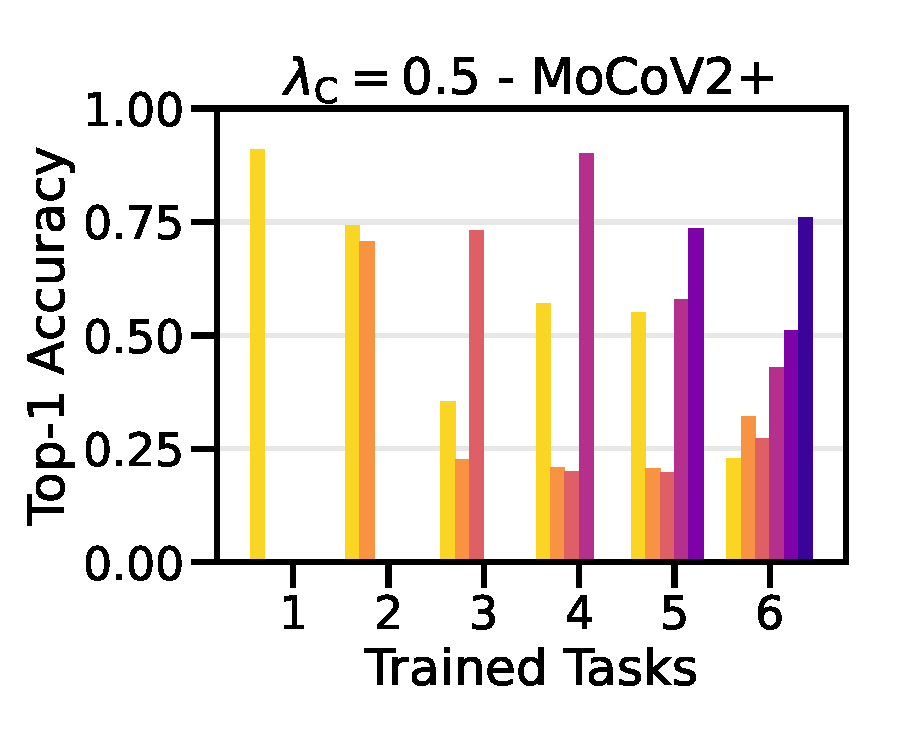
\includegraphics[width=0.32 \linewidth ]{figures_new/Part_2/F4-WISDM2019-__lambda___mathrm_C__=0.5_-MoCoV2+-6Tasks-v2.pdf}
    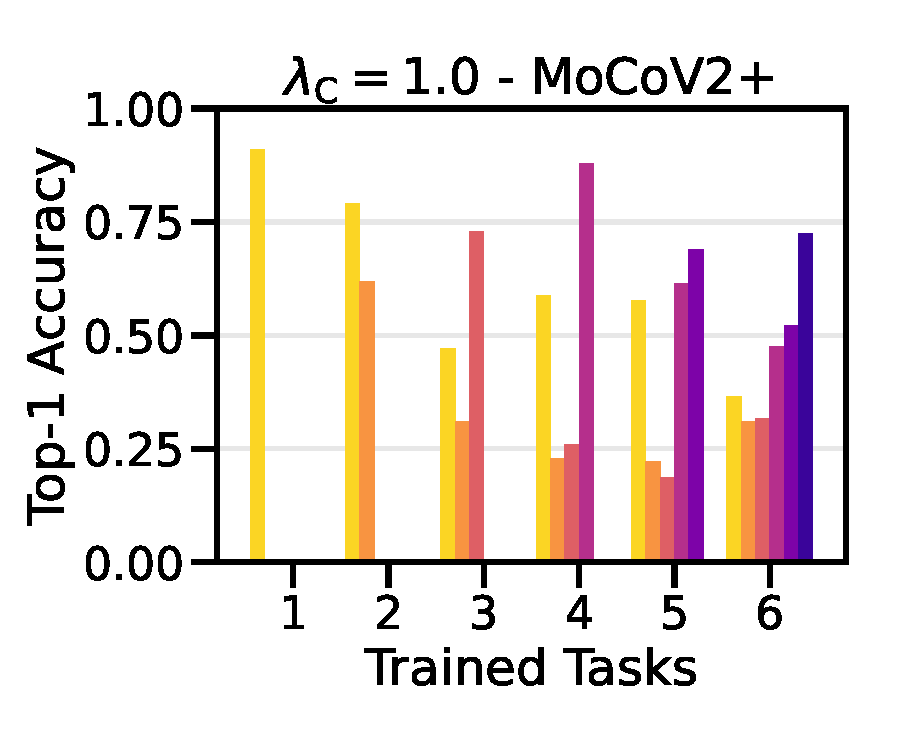
\includegraphics[width=0.32 \linewidth ]{figures_new/Part_2/F4-WISDM2019-__lambda___mathrm_C__=1.0_-MoCoV2+-6Tasks-v2.pdf}
    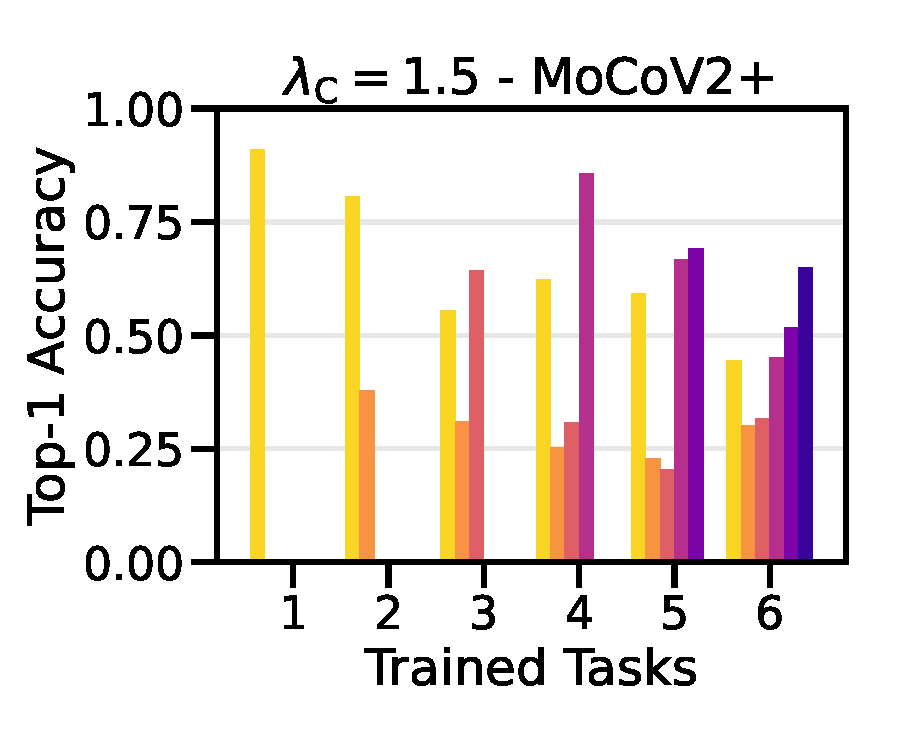
\includegraphics[width=0.32 \linewidth ]{figures_new/Part_2/F4-WISDM2019-__lambda___mathrm_C__=1.5_-MoCoV2+-6Tasks-v2.pdf} \\
    \vspace{-0.05in}
    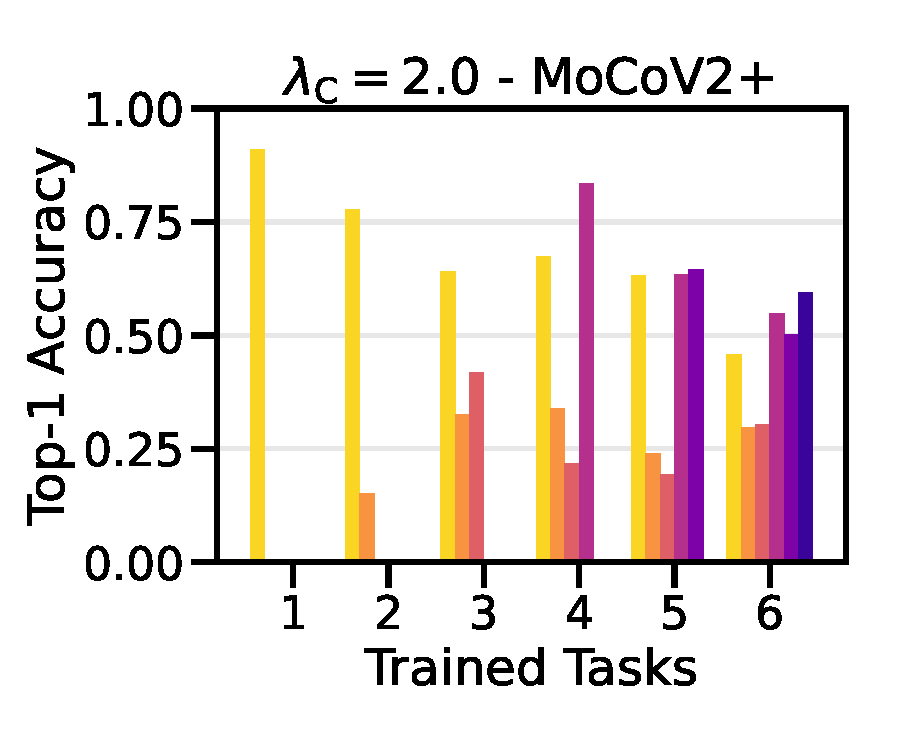
\includegraphics[width=0.32 \linewidth ]{figures_new/Part_2/F4-WISDM2019-__lambda___mathrm_C__=2.0_-MoCoV2+-6Tasks-v2.pdf}
    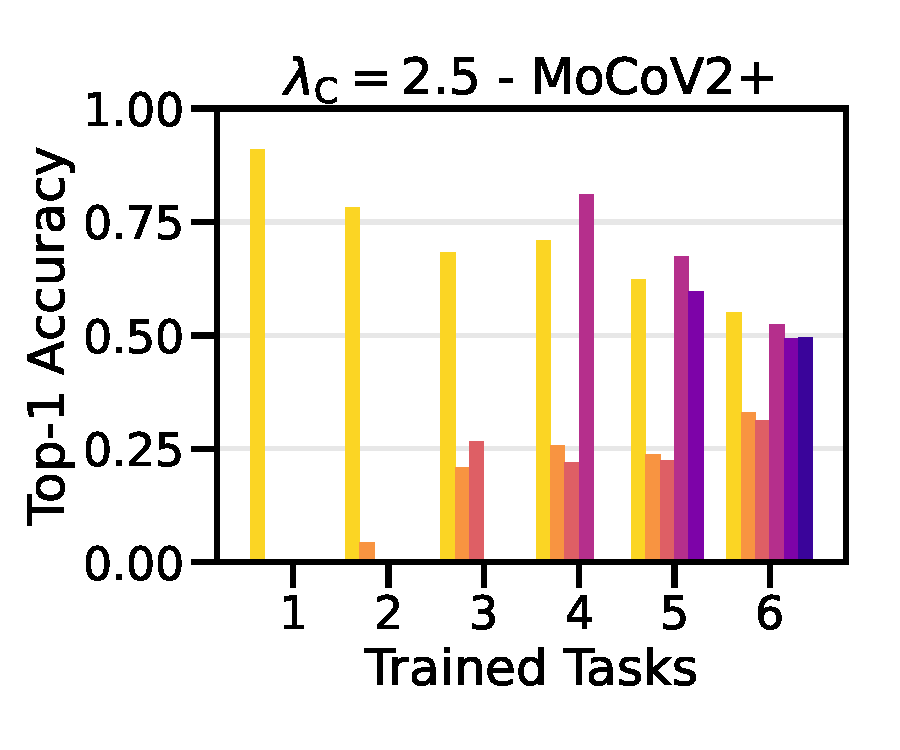
\includegraphics[width=0.32 \linewidth ]{figures_new/Part_2/F4-WISDM2019-__lambda___mathrm_C__=2.5_-MoCoV2+-6Tasks-v2.pdf} \\
    \vspace{-0.05in}
    
\includegraphics[width=0.65 \linewidth ]{figures_new/Part_1/F4-WISDM2019-6Tasks-v2_legend.pdf}
    \vspace{-0.1in}
    \caption{Detailed breakdown of performance over tasks with constant importance coefficients. Fine-grained accuracy is shown for every additional task with different importance coefficients.}
    \label{fig:kaizen_performance_per_task_constant_lamb}
\end{figure}

We conducted an additional set of experiments exploring the effect of this hyperparameter on the performance of the model across time while all other hyperparameters remain unchanged for Kaizen. Fig. \ref{fig:kaizen_general_performance_constant_lamb} and \ref{fig:kaizen_performance_per_task_constant_lamb} illustrate the changes in performance when we set the value of $\lambda_{\mathrm{C}}$ to 0.5, 1.0, 1.5, 2.0, and 2.5 (additional visualisation can be found in Appx.~\ref{subsection:additional_results}). From Fig.~\ref{fig:kaizen_performance_per_task_constant_lamb}, we can see that with lower values of $\lambda_{\mathrm{C}}$, the model tends to have higher accuracy in new tasks right after they have been trained on them, which is similar to that of CaSSLe. Higher values of $\lambda_{\mathrm{C}}$, on the other hand, force the model to retain knowledge on older tasks, which matches our understanding of this hyperparameter.

We also observe a trend here: even though higher values of $\lambda_{\mathrm{C}}$ forces the model to retain more knowledge (see Fig.~\ref{fig:kaizen_performance_per_task_constant_lamb}, where the performance on task 1, denoted by T1, remains high throughout all steps for $\lambda_{\mathrm{C}}=2.5$), the overall performance of the model ends up lower in the long run (see Fig.~\ref{fig:kaizen_general_performance_constant_lamb}). This can be counter-intuitive, but explainable by inspecting $\lambda_{\mathrm{C}}$: a high value of $\lambda_{\mathrm{C}}$ sacrifices new task learning for knowledge retention, and this effect \emph{compounds} over time. Performance on the initial task (task 1) is kept at the highest priority when using a high $\lambda_{\mathrm{C}}$, while all other tasks suffer as the model is being trained. This is reflected in Fig.~\ref{fig:kaizen_performance_per_task_constant_lamb}, where the performance on tasks 2, 3, 4, 5, and 6 starts off with a much lower value when using $\lambda_{\mathrm{C}}=2.5$ compared to $\lambda_{\mathrm{C}}=0.5$. Since the goal of continual learning is to maintain high performance on \emph{all} trained tasks over time, such a trade-off can hurt the overall performance.

We hypothesise that a \emph{progressive} importance coefficient can allow the model to balance knowledge retention and new task learning better than a constant value: as the model gets trained on more classes and tasks, the importance of knowledge retention should increase, and it should be proportional to the number of classes already learned compared to the number of new classes to be learned. To test this hypothesis, we designed a set of experiments where the importance coefficient is increased by a constant value after each task. We denote the setting where $\lambda_{\mathrm{C}}$ is set to $a$ initially, and increased by $b$ after each task as $\lambda_{\mathrm{C}}=a \oplus b$. That is, the importance coefficient at task $t$ is given by $\lambda_{\mathrm{C}}(t) = a + b \times (t - 1)$.
For example, the setting $\lambda_{\mathrm{C}}=1.0 \oplus 0.5$ will see values of $\lambda_{\mathrm{C}}$ being set to 1.0, 1.5, 2.0, 2.5, 3.0, and 3.5 for tasks 1, 2, 3, 4, 5, and 6 respectively, while the setting $\lambda_{\mathrm{C}}=1.0 \oplus 0.0$ is identical to that of a constant $\lambda_{\mathrm{C}}=1.0$.

\begin{figure}[t]
\begin{center}
   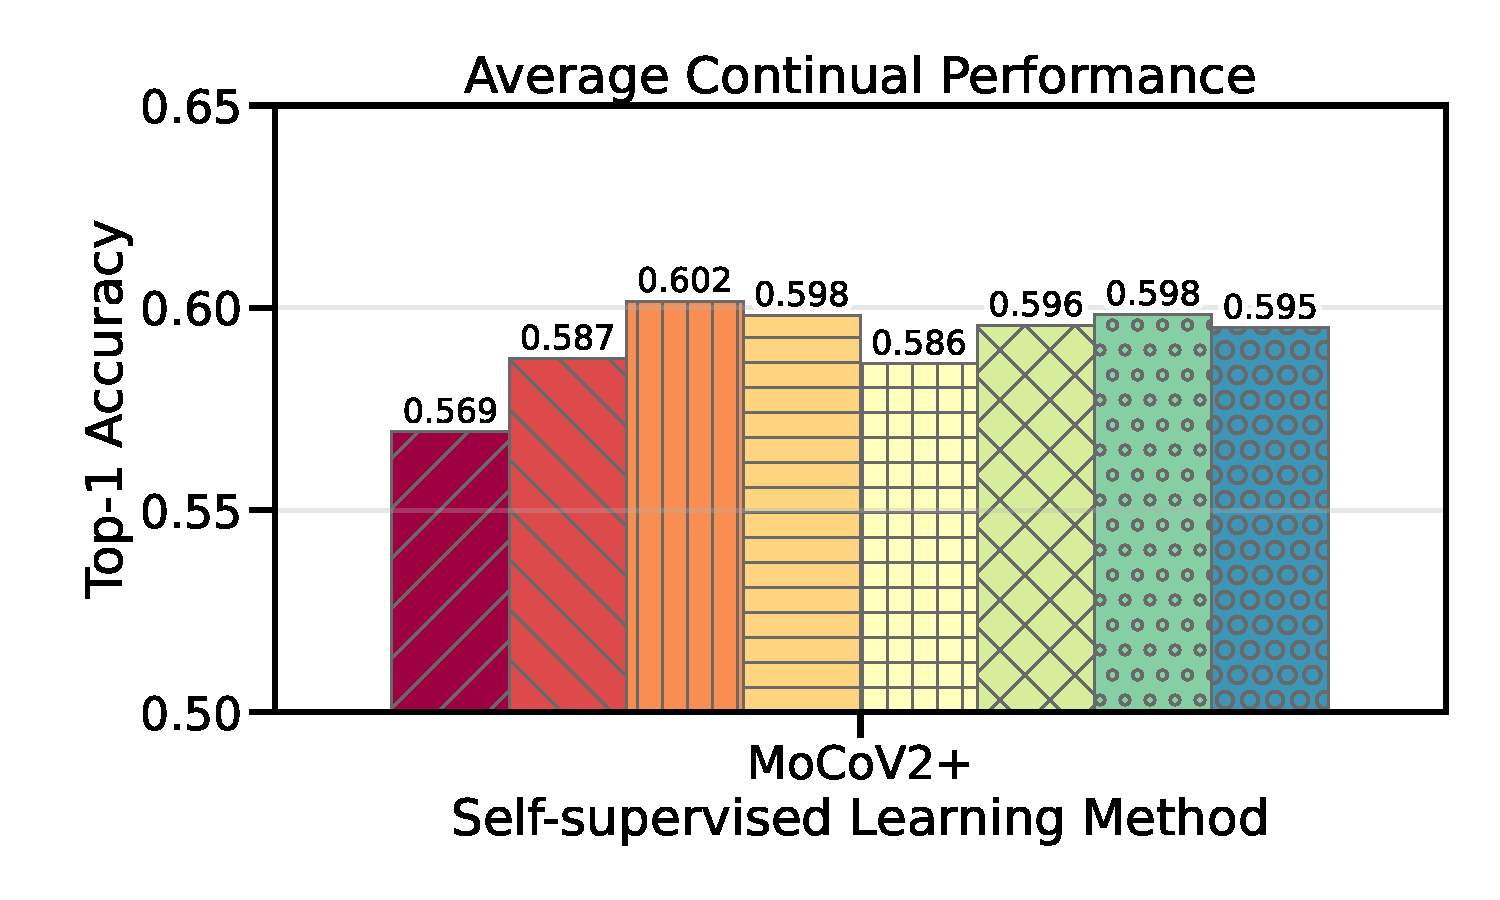
\includegraphics[width=0.49\linewidth]{figures_new/Part_3/F1-WISDM2019-6Tasks-Continual_Accuracy-v2.pdf}
   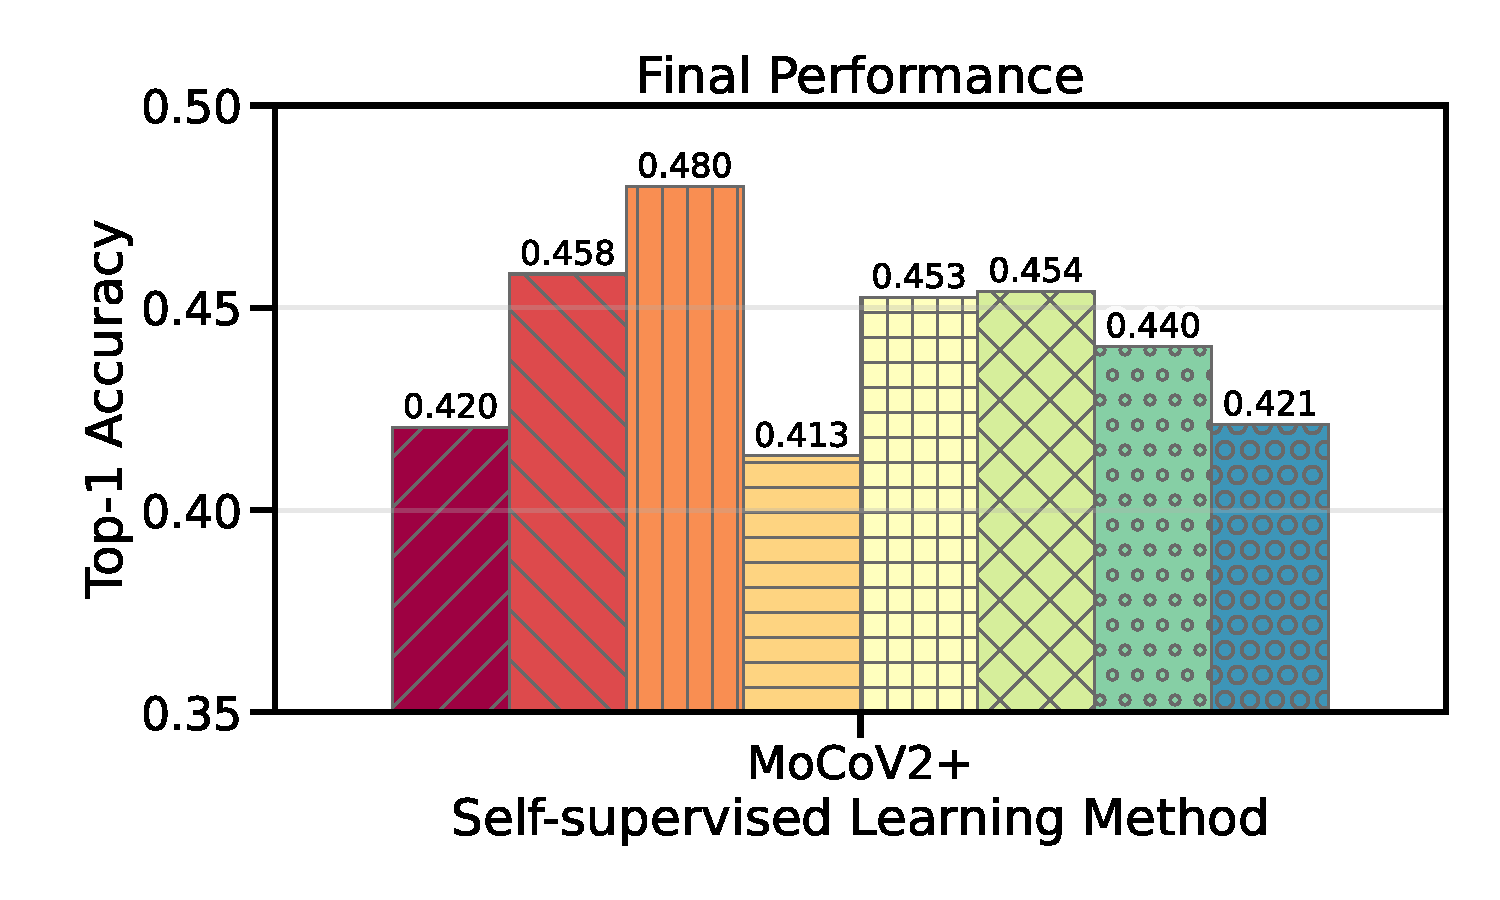
\includegraphics[width=0.49\linewidth]{figures_new/Part_3/F1-WISDM2019-6Tasks-Final_Accuracy-v2.pdf} \\
   \vspace{-0.05in}
   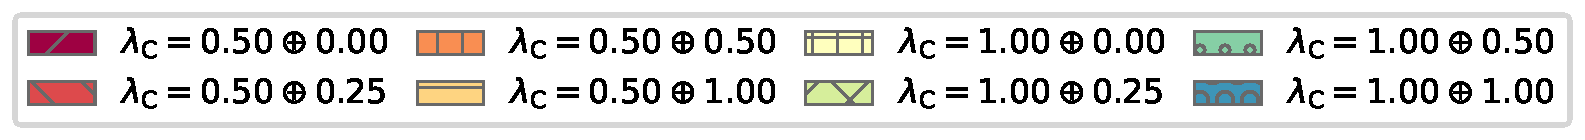
\includegraphics[width=0.9\linewidth]{figures_new/Part_3/F1-WISDM2019-6Tasks-v2_legend.pdf}
\end{center}
\vspace{-0.15in}
   \caption{Effects of progressive importance coefficients. The plot compares the aggregate performance metrics of models trained with the importance coefficient for the classifier set to different progressive values.}
   \label{fig:kaizen_general_performance_progressive_lamb}
       \vspace{-0.2in}
\end{figure}


\begin{figure}[ht]
    \centering
    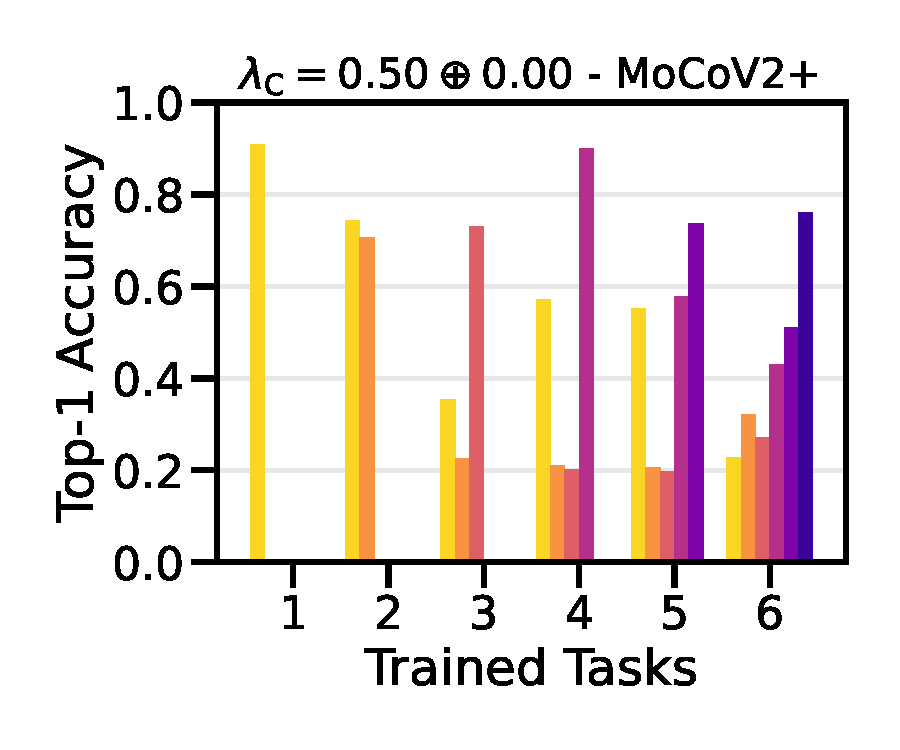
\includegraphics[width=0.24 \linewidth ]{figures_new/Part_3/F4-WISDM2019-__lambda___mathrm_C__=0.50_oplus0.00_-MoCoV2+-6Tasks-v2.pdf}
    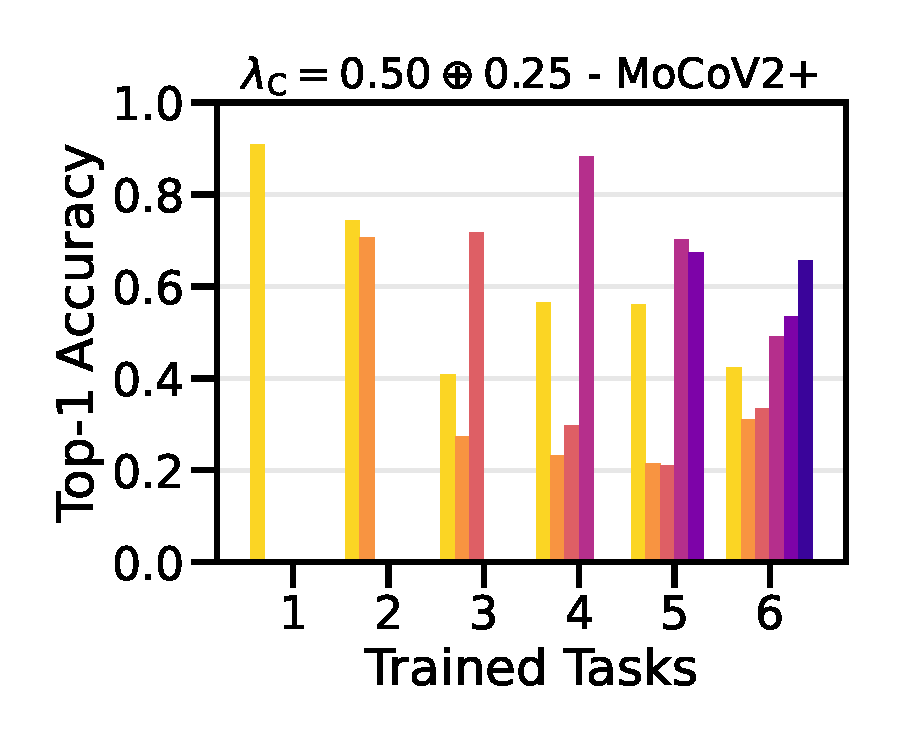
\includegraphics[width=0.24 \linewidth ]{figures_new/Part_3/F4-WISDM2019-__lambda___mathrm_C__=0.50_oplus0.25_-MoCoV2+-6Tasks-v2.pdf}
    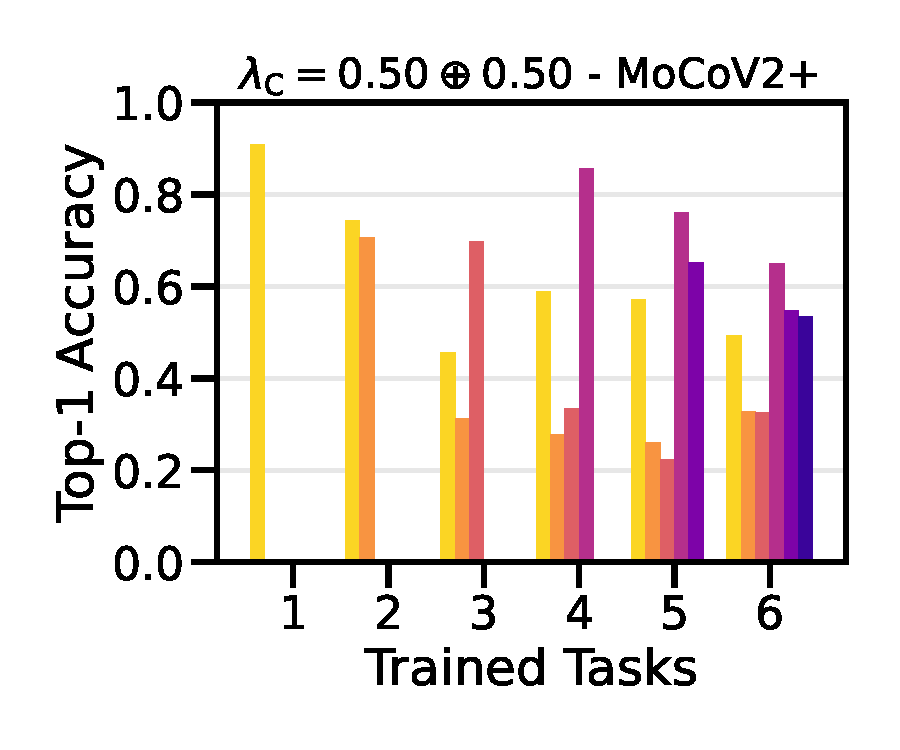
\includegraphics[width=0.24 \linewidth ]{figures_new/Part_3/F4-WISDM2019-__lambda___mathrm_C__=0.50_oplus0.50_-MoCoV2+-6Tasks-v2.pdf}
    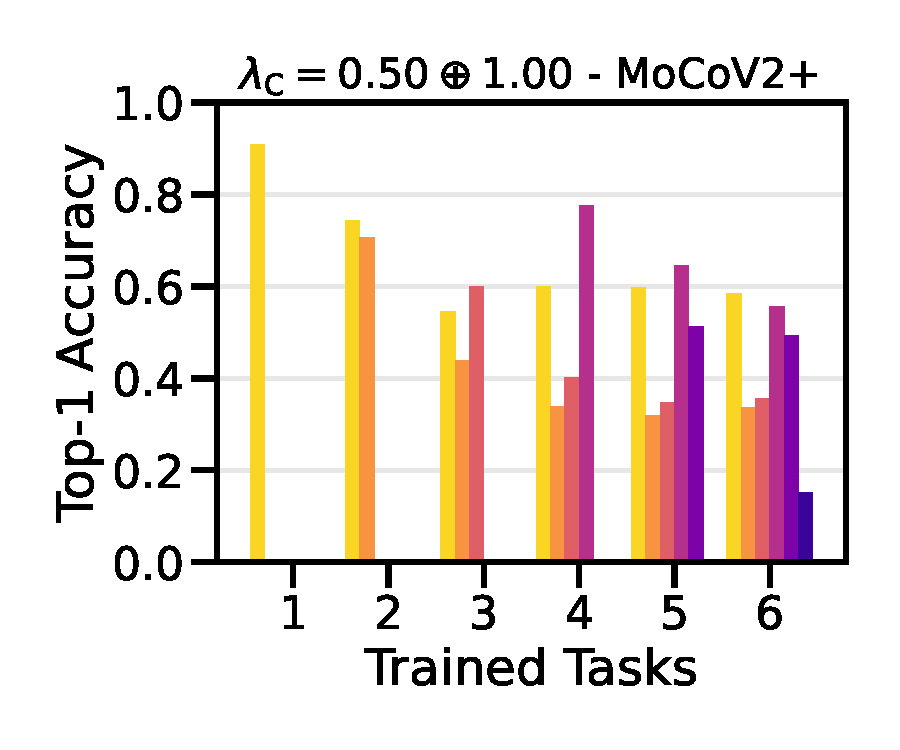
\includegraphics[width=0.24 \linewidth ]{figures_new/Part_3/F4-WISDM2019-__lambda___mathrm_C__=0.50_oplus1.00_-MoCoV2+-6Tasks-v2.pdf} \\
    \vspace{-0.05in}
    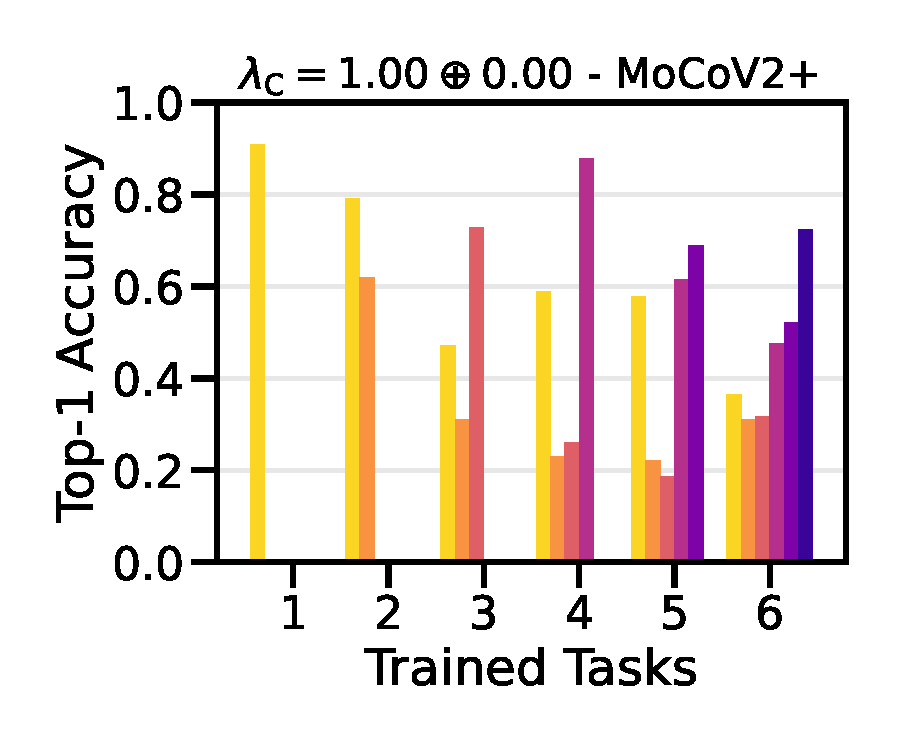
\includegraphics[width=0.24 \linewidth ]{figures_new/Part_3/F4-WISDM2019-__lambda___mathrm_C__=1.00_oplus0.00_-MoCoV2+-6Tasks-v2.pdf}
    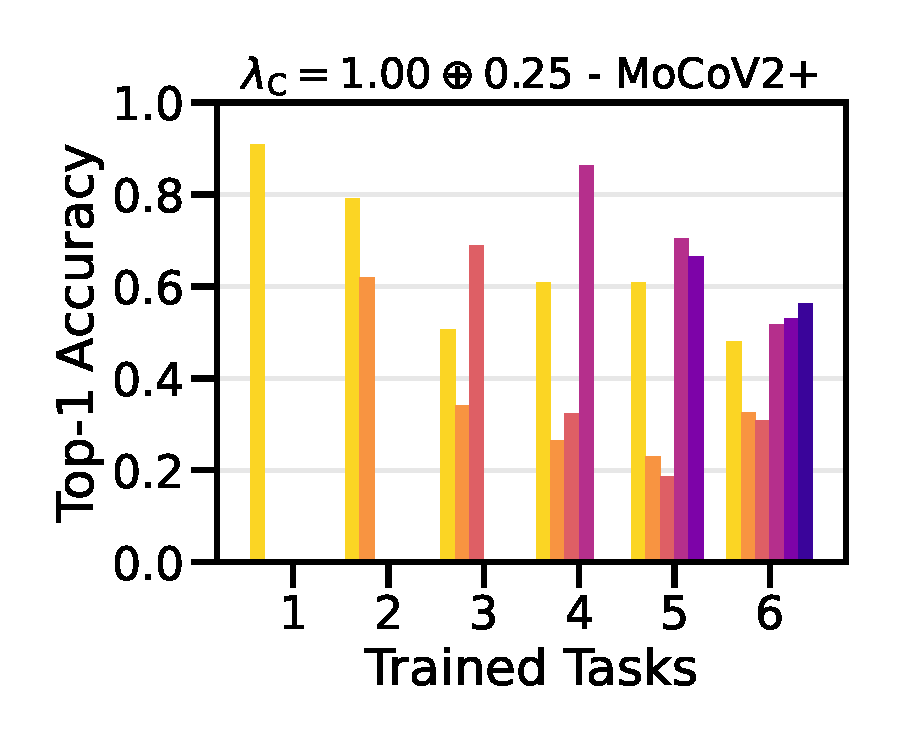
\includegraphics[width=0.24 \linewidth ]{figures_new/Part_3/F4-WISDM2019-__lambda___mathrm_C__=1.00_oplus0.25_-MoCoV2+-6Tasks-v2.pdf}
    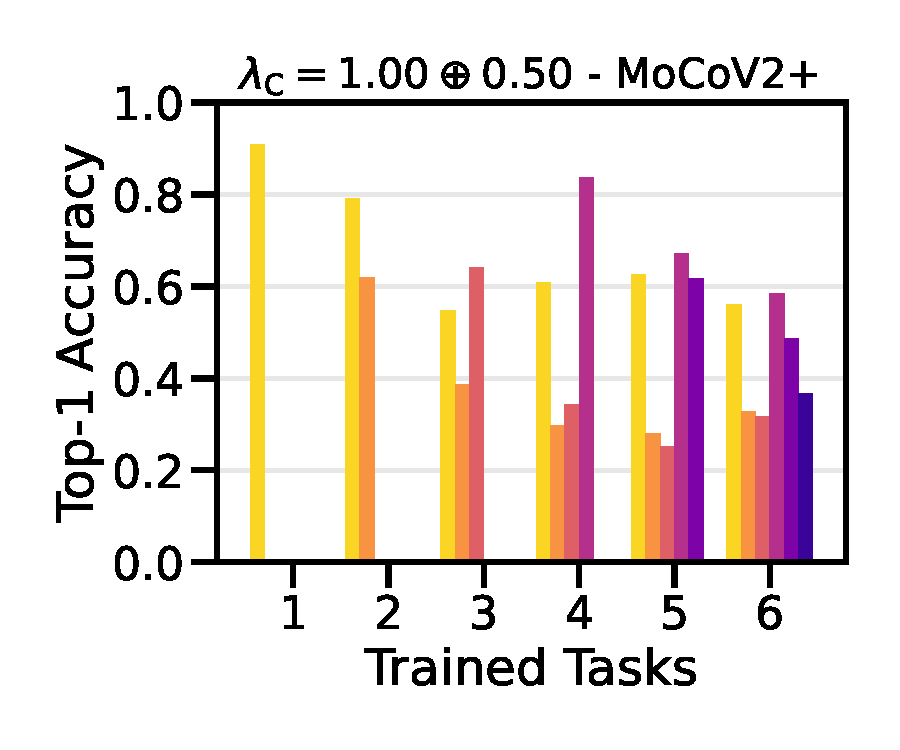
\includegraphics[width=0.24 \linewidth ]{figures_new/Part_3/F4-WISDM2019-__lambda___mathrm_C__=1.00_oplus0.50_-MoCoV2+-6Tasks-v2.pdf}
    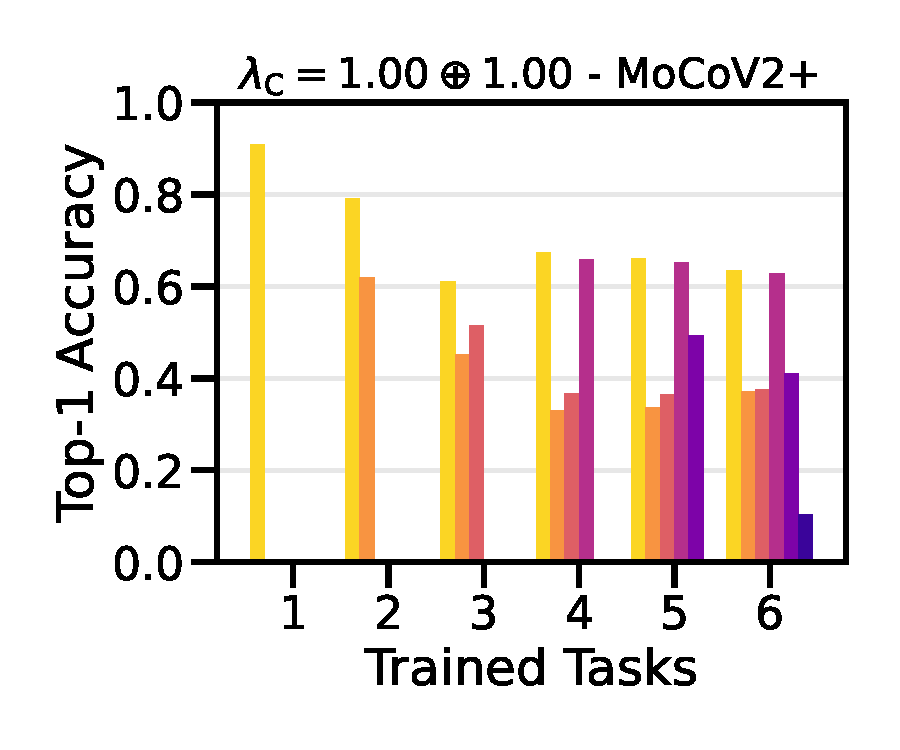
\includegraphics[width=0.24 \linewidth ]{figures_new/Part_3/F4-WISDM2019-__lambda___mathrm_C__=1.00_oplus1.00_-MoCoV2+-6Tasks-v2.pdf} \\
    \vspace{-0.05in}
    
\includegraphics[width=0.65 \linewidth ]{figures_new/Part_1/F4-WISDM2019-6Tasks-v2_legend.pdf}
    \vspace{-0.1in}
    
    \caption{Detailed breakdown of performance over tasks with progressive importance coefficients. Fine-grained accuracy is shown for every additional task with different importance coefficients.}
    \vspace{-0.2in}
    \label{fig:kaizen_performance_per_task_progressive_lamb}
\end{figure}

We conducted 8 additional experiments with different progressive importance coefficients: $\lambda_{\mathrm{C}}$ = $0.50 \oplus 0.00$, $0.50 \oplus 0.25$, $0.50 \oplus 0.50$, $0.50 \oplus 1.00$, $1.00 \oplus 0.00$, $1.00 \oplus 0.25$, $1.00 \oplus 0.50$, $1.00 \oplus 1.00$, and the results are shown in Fig.~
 \ref{fig:kaizen_general_performance_progressive_lamb} and \ref{fig:kaizen_performance_per_task_progressive_lamb} (additional visualisation can be found in Appx.~\ref{subsection:additional_results}).
From the detailed breakdown (see Fig.~\ref{fig:kaizen_performance_per_task_progressive_lamb}), we can verify our understanding: the performance on trained tasks remains almost unchanged at the last few tasks when the progressive factor is high (see the plots of $0.50 \oplus 1.00$ and $1.00 \oplus 1.00$). The use of a progressive factor allows the model to shift the focus from new task learning to knowledge retention over time. The results shown in Fig. \ref{fig:kaizen_general_performance_progressive_lamb} further support our hypothesis on proportional importance: with $\lambda_{\mathrm{C}}=0.50 \oplus 0.50$, which corresponds to scaling the importance of knowledge retention proportional to the number of tasks learned, the model can achieve the highest average continual performance and final performance. A higher value of $\lambda_{\mathrm{C}}=1.00 \oplus 1.00$ can still maintain high performance, but an increased coefficient at later steps hurts the performance of the final model. Other settings display a spectrum of performance with varying priorities given to knowledge distillation and current task learning. This set of results allows us to better explore the trade-off between knowledge retention and new task learning, a key aspect of continual learning.

